\documentclass[12pt,letterpaper]{article}

\usepackage[margin=1in]{geometry} % page margins & stuff
\usepackage{microtype} % improves font readability
\usepackage{yfonts}

\usepackage{hyperref}%adds pdf hyperlinks for document references (e.g., table of contents)
\usepackage{url} % nice url typesetting
\usepackage{textcomp}%used for \textrangle & similar--adds symbols for text environment
\usepackage{graphicx}%for pictures and stuff
\usepackage{subcaption}%needed for side-by-side pictures

\usepackage{multicol}%multicolumn stuff in tables
\usepackage{booktabs}%adds additional table commands (\toprule, etc.)
\usepackage{authblk}%changes the way \author{} works, adds \affiliation{} & similar

\usepackage{hanging}%allows us to use hanging paragraphs in the references section
\usepackage{xcolor}%enables use of colors
\newcommand{\email}[1]{%used to typeset emails in the 'title settings' section
  $\langle$\href{mailto:#1}{\nolinkurl{#1}}$\rangle$
}

\newcommand{\hl}[1] {%used to highlight text
{\color{red}#1}%
}

\title{Proposal for Enhanced Charlottesville Area Transit Mobile Application}
\author{Andrea Shaw \\ \email{rcs8vq@virginia.edu}}%
\affil{Department of Computer Science \\ University of Virginia}

\date{September 2016}

\begin{document}

\maketitle

\begin{abstract}

    A proposal is presented regarding aesthetic and functional improvements to
    the Charlottesville Area Transit (CAT) mobile app. A peer application and the
    community context surrounding the app are considered. Recommendations
    center on making the app more accessible to a wider community, and
    streamlining the graphical user interface for rapid information retrieval.
    Given that CAT serves a historic college town, the improvements suggested
    are believed to optimize route visualization and timing, while increasing
    revenue by recognizing more affluent customers
    (who are more likely than others to own a smartphone) along
    with the traditional working-class commuter base.


    \bigskip
    \noindent \emph{Keywords}: {\tt Charlottesville Area Transport, public transport, mobile app}
\end{abstract}

\vspace{5mm}

\begin{quote}
A developed country is not a place where the poor have cars. It's where the rich use public transport.

\raggedleft ---attributed to Enrique Pe\~{n}alosa, former Mayor of Bogot\'{a}, Colombia
\end{quote}

\section{Problem Definition}
In 2014, the Charlottesville Area Transit (CAT) organization commissioned a new
mobile app meant to help bus riders better understand their public
transportation options and reduce dependence on the outdated paper- and phone-based
timetable systems (NBC29 WVIR Charlottesville, 2014). Though basically
functional, the graphical user interface (GUI) of the mobile application leaves
much to be desired. Unlike its web-based counterpart (see Fig.~\ref{fig:cat_online})
the app provides no obvious way of obtaining arrival estimates for all of the
operational area's bus stops. Furthermore, it may crash or otherwise fail to
boot up on many devices. Though the app has received praise from public officials,
having been awarded the 2015 Governor's Technology Award
as a submission featuring "the strategic use of IT to
increase productivity, boost efficiency, and reduce overall operating costs"
(NBC29 WVIR Charlottesville, 2015),
there still remains work to be done.


\begin{figure}[th!]
    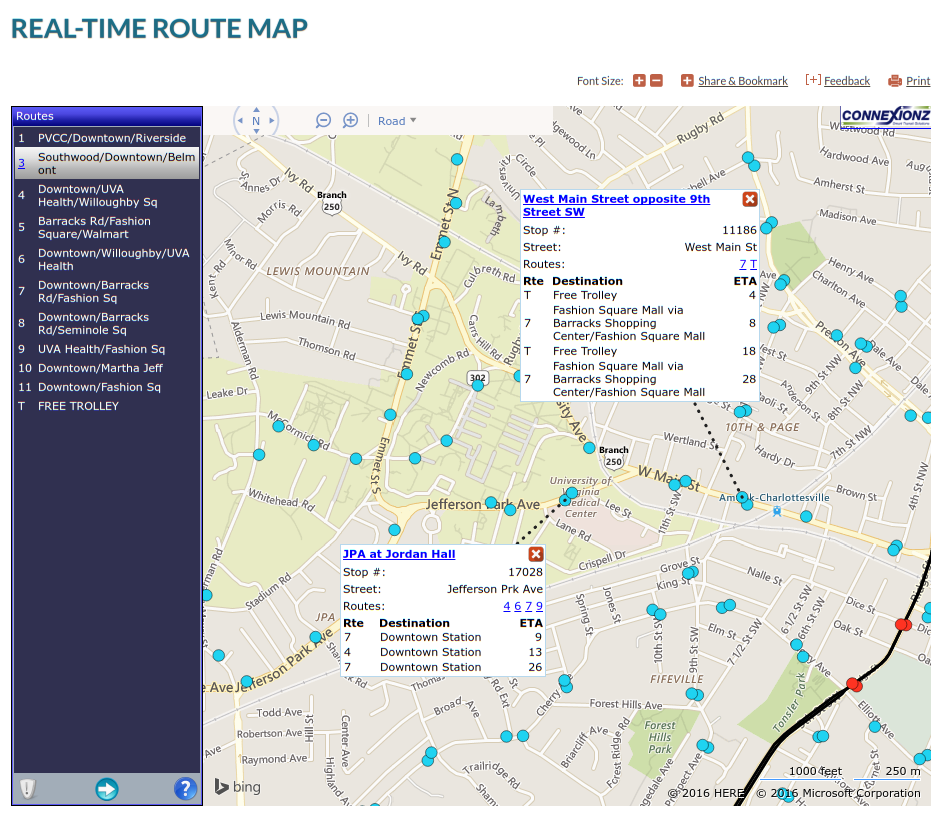
\includegraphics[width=\textwidth]{CAT_online}
    \caption{
        \label{fig:cat_online}
        The CAT ``Real-Time Route Map'', a website designed for desktop
        use that shows a system map, complete with all stops in the service area, along with
        timetable options (City of Charlottesville, n.d.).
    }
\end{figure}

By introducing the arrival estimate system and improving app stability and
design, it is hoped that the application will better serve the
Charlottesville community and increase the individual's access to public
transit. College towns like Charlottesville are relatively unique in that they
often feature a close relationship between schools and the local and municipal
governments that surround them. A result of this mutually-beneficial
arrangement, we find that many college town mass transit options feature unique
challenges.

In the case of Charlottesville, where two primary bus
systems\footnote{The University Transit System (UTS) serves primarily students
and employees of the University of Virginia. The territory covered by
Charlottesville Area Transit overlaps in many cases with that of the UTS---the
CAT Free Trolley, for example, connects the University area to the Downtown
Mall. CAT is also funded, in part, by the University of Virginia (CAT, 2011,
p.~6), and students and ID-carrying employees of the University of Virginia may
ride CAT buses free of charge.} intersect within city limits, the bus-riding
population is significantly more diverse in age and income-level than the country at large.
Whereas riders on CAT bus routes are a steady mix of work-commuters, students,
and shoppers of varying ethnic background (CAT, 2011, p.~48--49), Taylor \&
Morris (2015) contend that bus transit in the United States is generally skewed
towards commuters and minority riders. The limited availability of parking and
other contraindications for travel by car result in a heavy reliance of city
residents from all backgrounds on the bus transit system. It is therefore expedient that
the area continue to invest in the convenience of travel by mass transit for all of
its citizens---their livelihood depends on it.

The improvements suggested in this document to the existing CAT mobile app are hoped to address a broad cross-section
of the community, providing enhanced utility to all users within.

\section{Prototype Brainstorming}
Our proposal suggests implementing minor fixes and \ae{}sthetic tweaks to the existing mobile app. The version current at the time of writing (Charlottesville Area Transit, release 3.8) is displayed in Fig.~\ref{fig:cat_mobile}

\begin{figure}[ph!]
\centering
\begin{subfigure}{.5\textwidth}
  \centering
  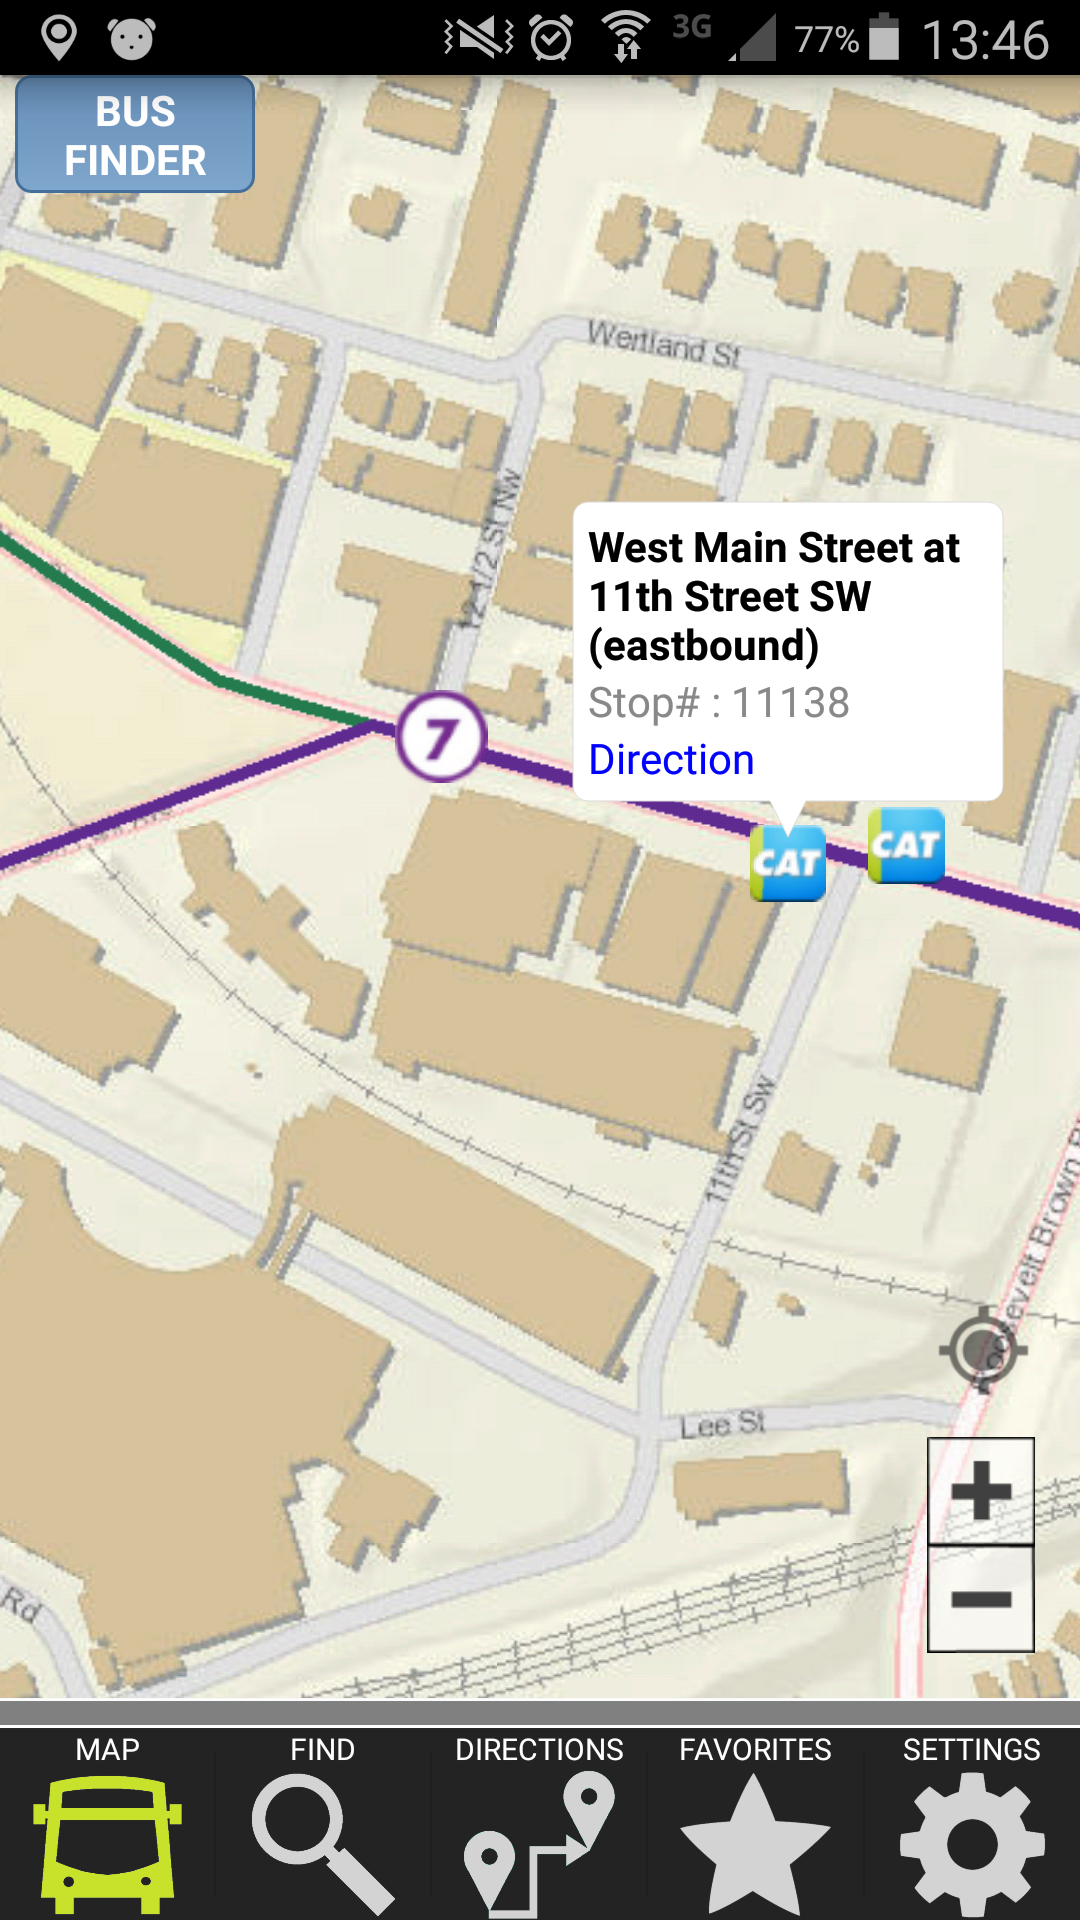
\includegraphics[width=.9\linewidth]{CAT_mobile_1}
  \caption{View of a bus route, stop selected}
  \label{fig:cat_mobile_1}
\end{subfigure}%
\begin{subfigure}{.5\textwidth}
  \centering
  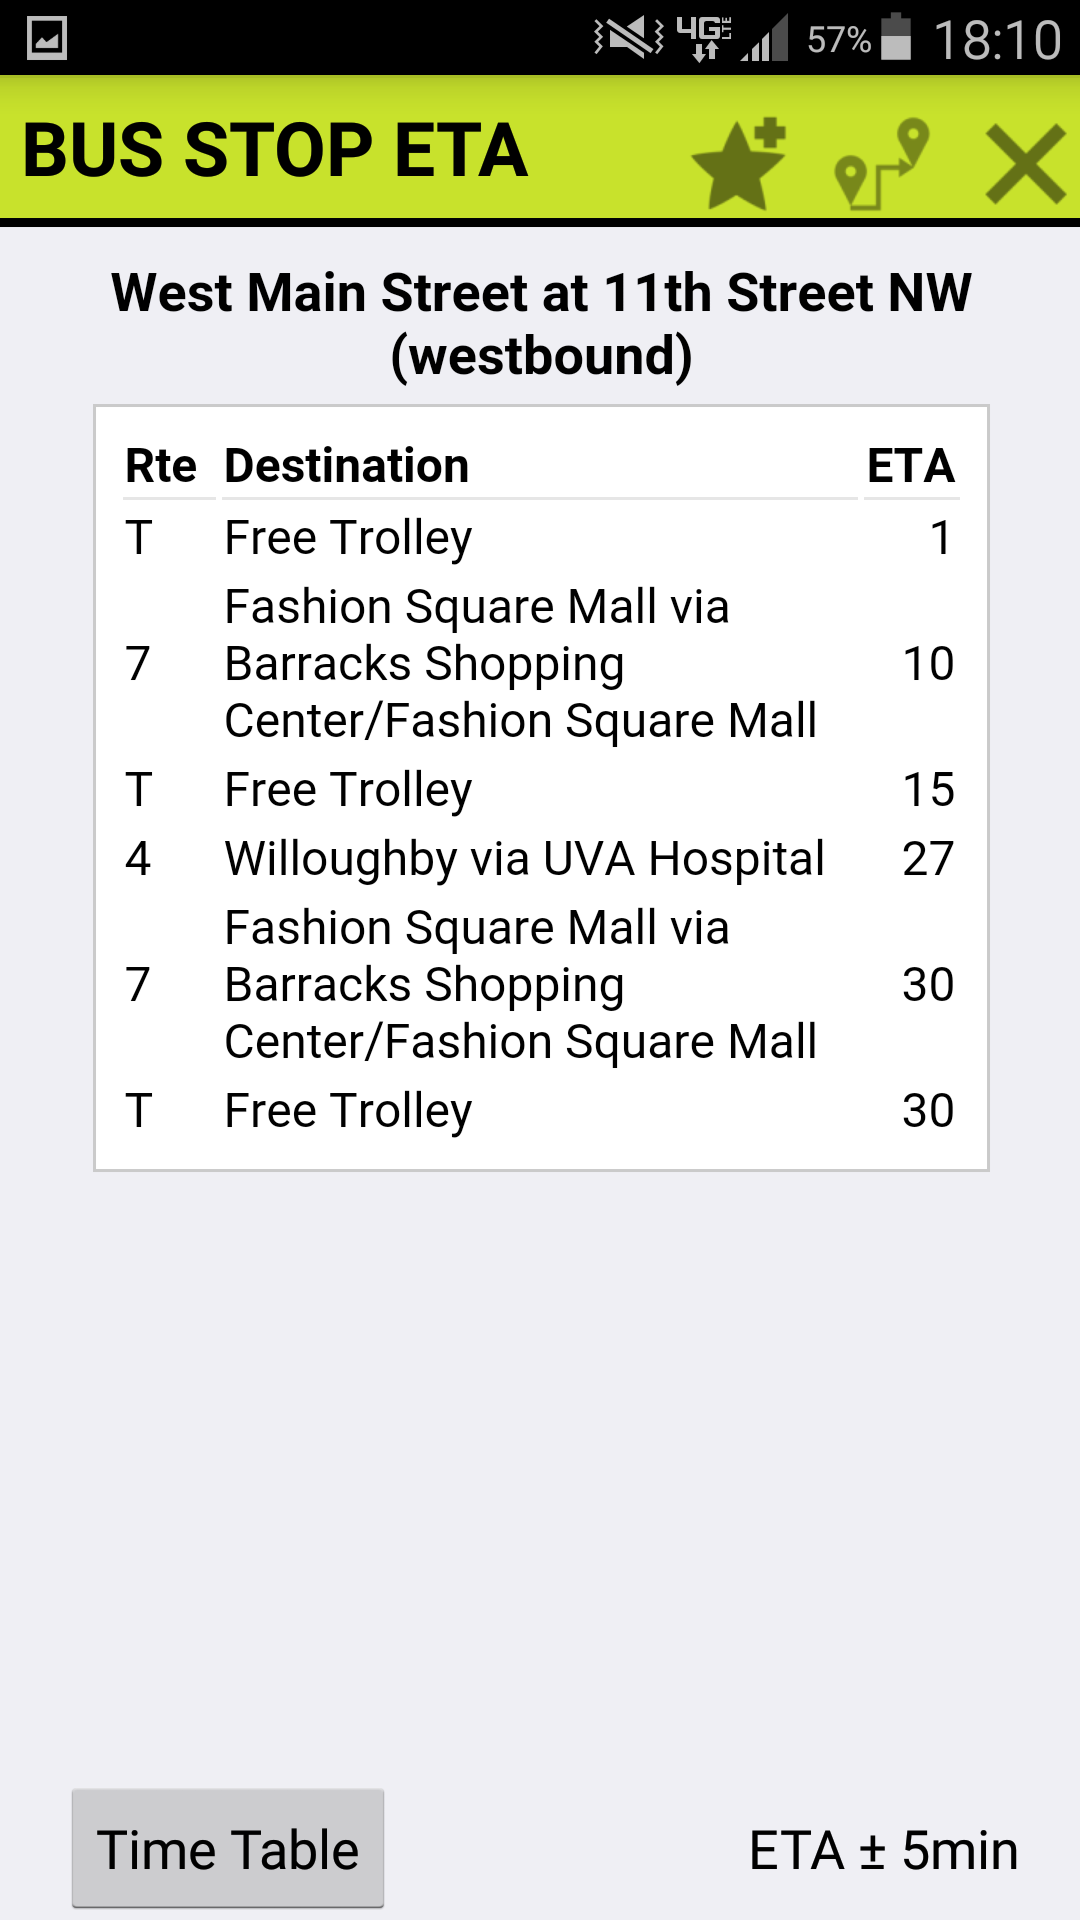
\includegraphics[width=.9\linewidth]{CAT_mobile_2}
  \caption{View of a timetable for the stop}
  \label{fig:cat_mobile_2}
\end{subfigure}
\caption{The Charlottesville Area Transit mobile app, depicted on a Samsung
    Galaxy S4 running Android Lollipop (version 5.0.1). Published by the City of Charlottesville (2016).}
\label{fig:cat_mobile}
\end{figure}

We will categorize this proposal into three areas of development.

\subsection{Modernization of GUI}
Though the current graphical user interface (GUI) for the mobile app is
generally quite functional, some minor cosmetic tweaks are advisable in order
to reduce user cognitive load necessary in learning the application for the
first time. For example, the button display bar at the bottom of the screen
that allows one to switch from one widget to another lacks demarcated borders
between neighboring elements. Additionally, the bar is not readily apparent to
the end user as a functional---they may appear to be part of the route
visualization above.

Our proposed solution to this problem is to redesign these
buttons natively; that is, to utilize the host operating system's pre-existing
(Android, iOS, or other) design features to best familiarize the user with the
app. If funding permits, developers might add on to this integration by
introducing phone notifications when a bus is about to arrive at the
current stop or left-right swiping to switch between one widget and the next.

\subsection{Lessons to Learn from Peer Software}
In this section, we will present the TransLoc (2015) mobile app as a point of
comparison. The TransLoc app is designed to perform the same overall
function as the CAT app, and is is recommended by the University of Virginia
to students as a way of visualizing their University Transit Service routes.

A quick comparison of the apps shows some distinct advantages to either app.
For one, the CAT app features much building shapes and more map features,
perhaps making it more useful to travelers navigating city streets on foot.
However, the TransLoc app details stops in a much more effective way than
the CAT app. Points of transfer between two or more different bus lines are
visualized using a pie chart, where a circle is evenly divided into colors
representing each route. The CAT app requires to the user to go through the
additional steps of twice tapping on a CAT icon to reveal the timetable,
showing all available buses through that stop. No visual aid is provided in
the application to show transfer points on the system map.

Because the transit system is inherently time-based, the additional steps
necessary to view stop information and time tables in the CAT app present
a particularly inefficient solution to the end user's needs. The goal of
the CAT app would be better met by implementing a combined stop information/%
timetable interface, as found in Fig.~\ref{fig:TL_mobile_2}.

Along a similar vein of logic, we find in Fig.~\ref{fig:cat_mobile_1} that the
CAT app fails to adequately depict shared routes---stop \textnumero{}11129 is
shared by both Route 7 and the Free Trolley, yet only Route 7 is shown
intersecting with it on the map. In contrast, TransLoc (refer to
Fig.~\ref{fig:TL_mobile_1}) solves this problem by using dashed lines of
alternating color to demonstrate that both routes travel past a given stop.

\begin{figure}[ph!]
\centering
\begin{subfigure}{.5\textwidth}
  \centering
  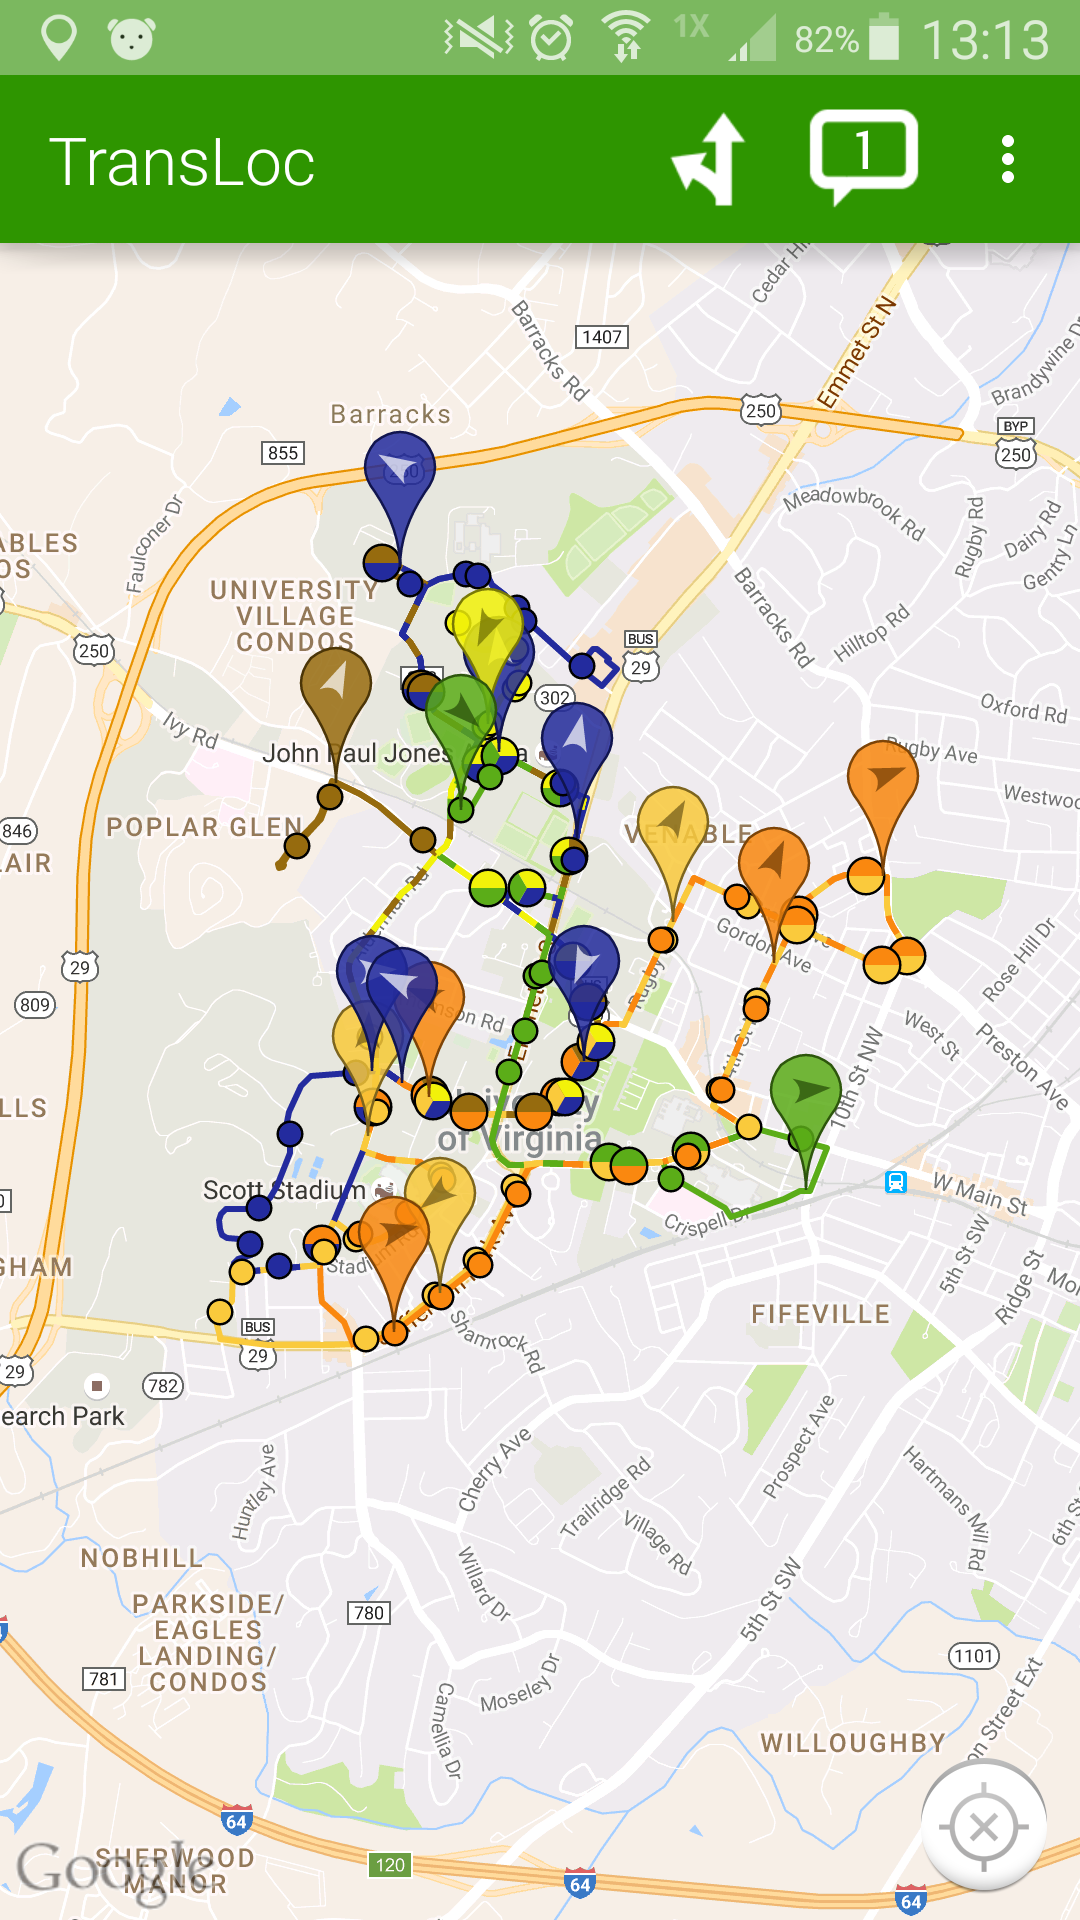
\includegraphics[width=.9\linewidth]{TL_mobile_1}
    \caption{Visualization of the University Transit System}
  \label{fig:TL_mobile_1}
\end{subfigure}%
\begin{subfigure}{.5\textwidth}
  \centering
  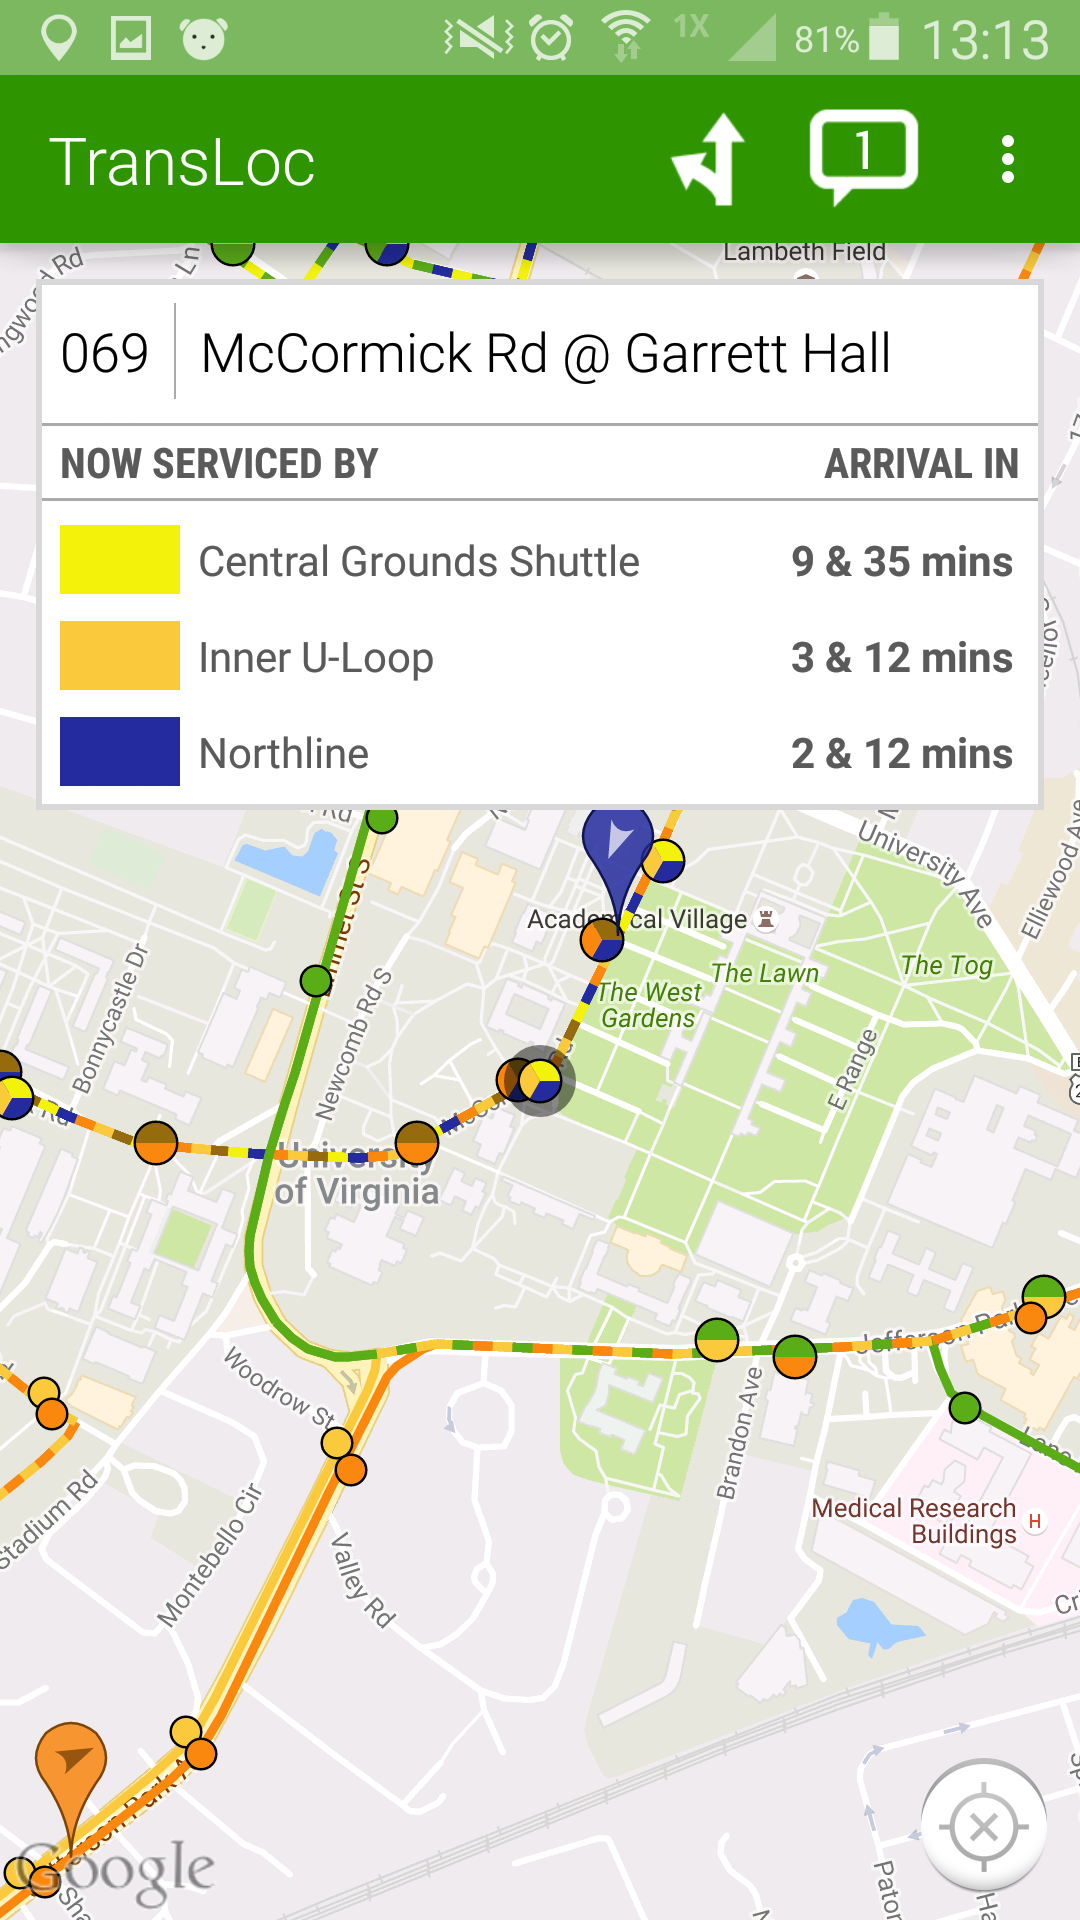
\includegraphics[width=.9\linewidth]{TL_mobile_2}
  \caption{View of a timetable for a specific stop}
  \label{fig:TL_mobile_2}
\end{subfigure}
    \caption{The TransLoc Transit Visualization mobile app, depicted on a Samsung Galaxy S4 running Android Lollipop (version 5.0.1). University of Virginia--UTS routes shown. Published by TransLoc (2015).}
\label{fig:TL_mobile}
\end{figure}

\subsection{Application Stability}
From anecdotal evidence, it appears that the CAT mobile app tends to freeze on
a loading screen or crash entirely at certain points. The cause is believed to be transferring from one networked access point to another, or from Wi-Fi to mobile data. Further quality assurance ought to be implemented subject to improved source code access.

\section{Expected Results}
We believe that implementing these suggested changes will significantly enhance
the user experience and improve access to public transit---especially amongst
those unfamiliar with the area, where easy to follow transportation directions
are key to successful tourism. As it stands currently, the Charlottesville Area
Transit app is rated at 4.0 out of 5.0 stars on the Google Play Store. An improved
app is likely to garner more positive reviews, which in turn will effect in
increased downloads and revenue streams.

Taylor \& Morris (2015) suggest that transit generally acts at a low level of
cost-effectiveness. By including not only transit typical customers, who tend
to be less affluent, but tourists and students in the target audience, one may
expect revenue to increase. Tourists tend to spend more money on more trips
than do commuters, who are more likely to purchase several days' worth of rides
at a time; and an increased student-rider population provides CAT with more
bargaining power with the University of Virginia and/or Piedmont Virginia
Community College, who subsidize their students' tickets.

In short, accepting this proposal is expected to increase customer satisfaction,
improve access to public transit options, and raise additional revenue.

\section{Acknowledgments}
The author wishes to recognize Luther 29 WVIR
 74 Charlottesville, 2015)
University of Virginia, for his seminars introducing basic
cognitive load theory, which heavily influenced the changes suggested in this
proposal.

\section{Honor Code}
On my word of honor, I have neither given nor received any unauthorized aid on this assignment.
\begin{center}
    Andrea Shaw\qquad {\hrulefill} \qquad 2016--08--25
\end{center}

\section{References}
\hangparas{1cm}{1}
Charlottesville Area Transit (2011, May). Transit Development Plan: Fiscal Years 2012--2017. Retrieved from \href{http://drpt.virginia.gov/media/1482/charlottesville-area-transit.pdf}{\tt http://drpt.virginia.gov/media/1482/charlottesville-area- \\
transit.pdf}.

City of Charlottesville (n.d.). Real-time Route Map. Retrieved from \href{http://www.charlottesville.org/departments-and-services/city-services/charlottesville-area-transit-cat/real-time-route-map}{\tt http:// \\
charlottesville.org/departments-and-services/ciity-services/ \\
charlottesville-area-transit-cat/real-time-route-map}.

City of Charlottesville (2016, 23 May). Charlottesville Area Transit (version 3.8) [Mobile application software]. Retrieved from \url{https://play.google.com/store/apps/details?id=com.cville.cattail}.

NBC29 WVIR Charlottesville (2014, 28 February). CAT riders can monitor bus status with new app. Retrieved online from \url{http://www.nbc29.com/story/24856561/cat-riders-can-monitor-bus-status-with-new-app}.

NBC29 WVIR Charlottesville (2015, 25 September). Development of CAT's mobile app wins technology award. Retrieved online from \url{http://www.nbc29.com/story/30009163/development-of-cats-mobile-app-wins-technology-award}.

Taylor, B.D. \& Morris, E.A. Transportation (2015) Public transportation objectives and rider demographics:
are transit’s priorities poor public policy? \emph{Transportation}, 42, 347--367. doi:10.1007/s11116-014-9547-0

TransLoc (2015, 27 April). TransLoc transit visualization [Mobile application software]. Retrieved from \url{https://play.google.com/store/apps/details?id=com.transloc.android}.
\end{document}

